\chapter{User Guide}
\label{ch:user}

\section{How To}

A user types a movie name and gets the details of the searched movie and top 10 recommendations according to the searched movie, if the search movie exists in our database. Otherwise the user receives a message that this movie is not in our database. If the user clicks on one of the recommended movies, the system shows the details and recommendations according to the clicked movie.

\section{Devices}

Our system has a responsive user interface for desktop, mobile portrait, mobile landscape, and iPad.

\subsection{Desktop}

Following figures show our project for the desktop. Figure \ref{fig:laptop-1} shows the first page when we load the website, the user searches the movie in the search bar and clicks the search button. If the searched movie exists, it shows the movie details and recommendations according to the searched movie as shown in Figure \ref{fig:laptop-2}. Otherwise it shows the message that the movie searched does not exist in our database as shown in Figure \ref{fig:laptop-error}.

\begin{figure}[ht]
	\centering
  	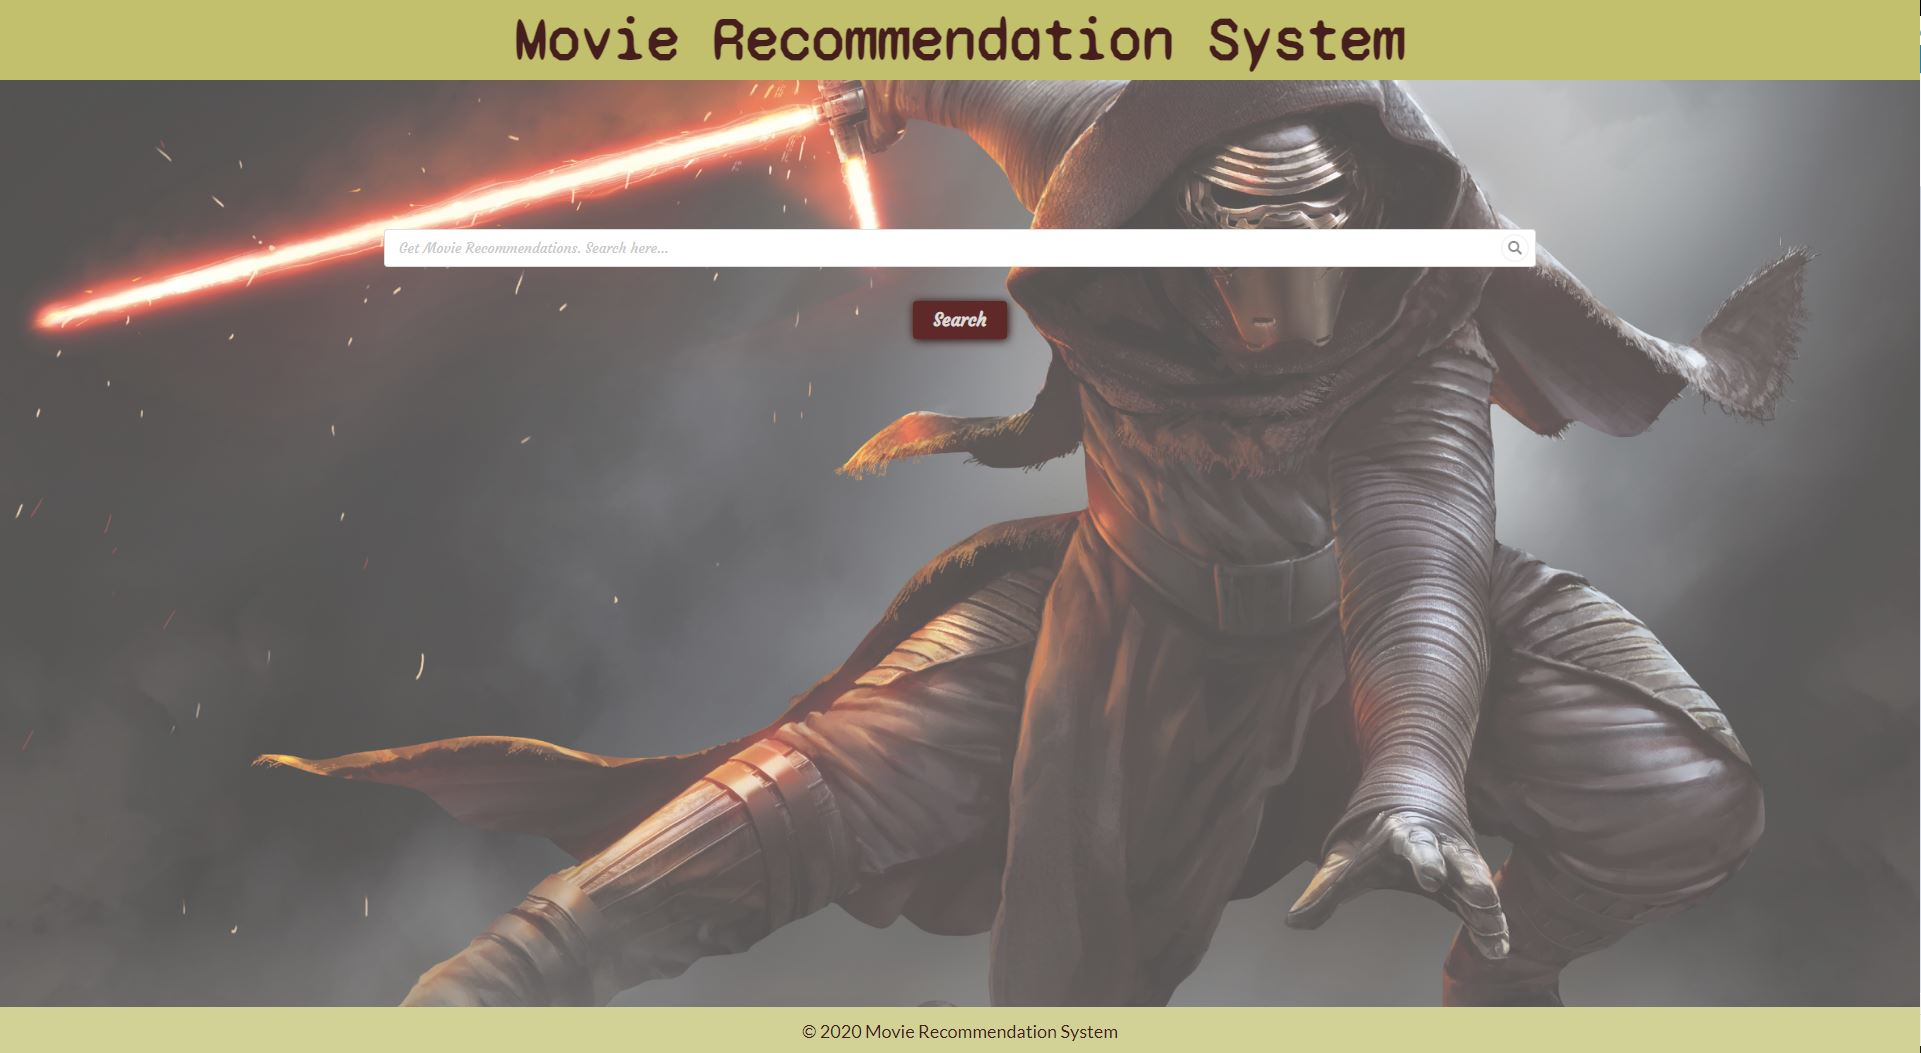
\includegraphics[width=1.0\textwidth]{images/laptop_1.JPG}
	\caption{\textbf{Screenshot of First Page on Desktop.} This figure shows the first page, when we load the website.}
  	\label{fig:laptop-1}
\end{figure}

\begin{figure}[ht]
	\centering
  	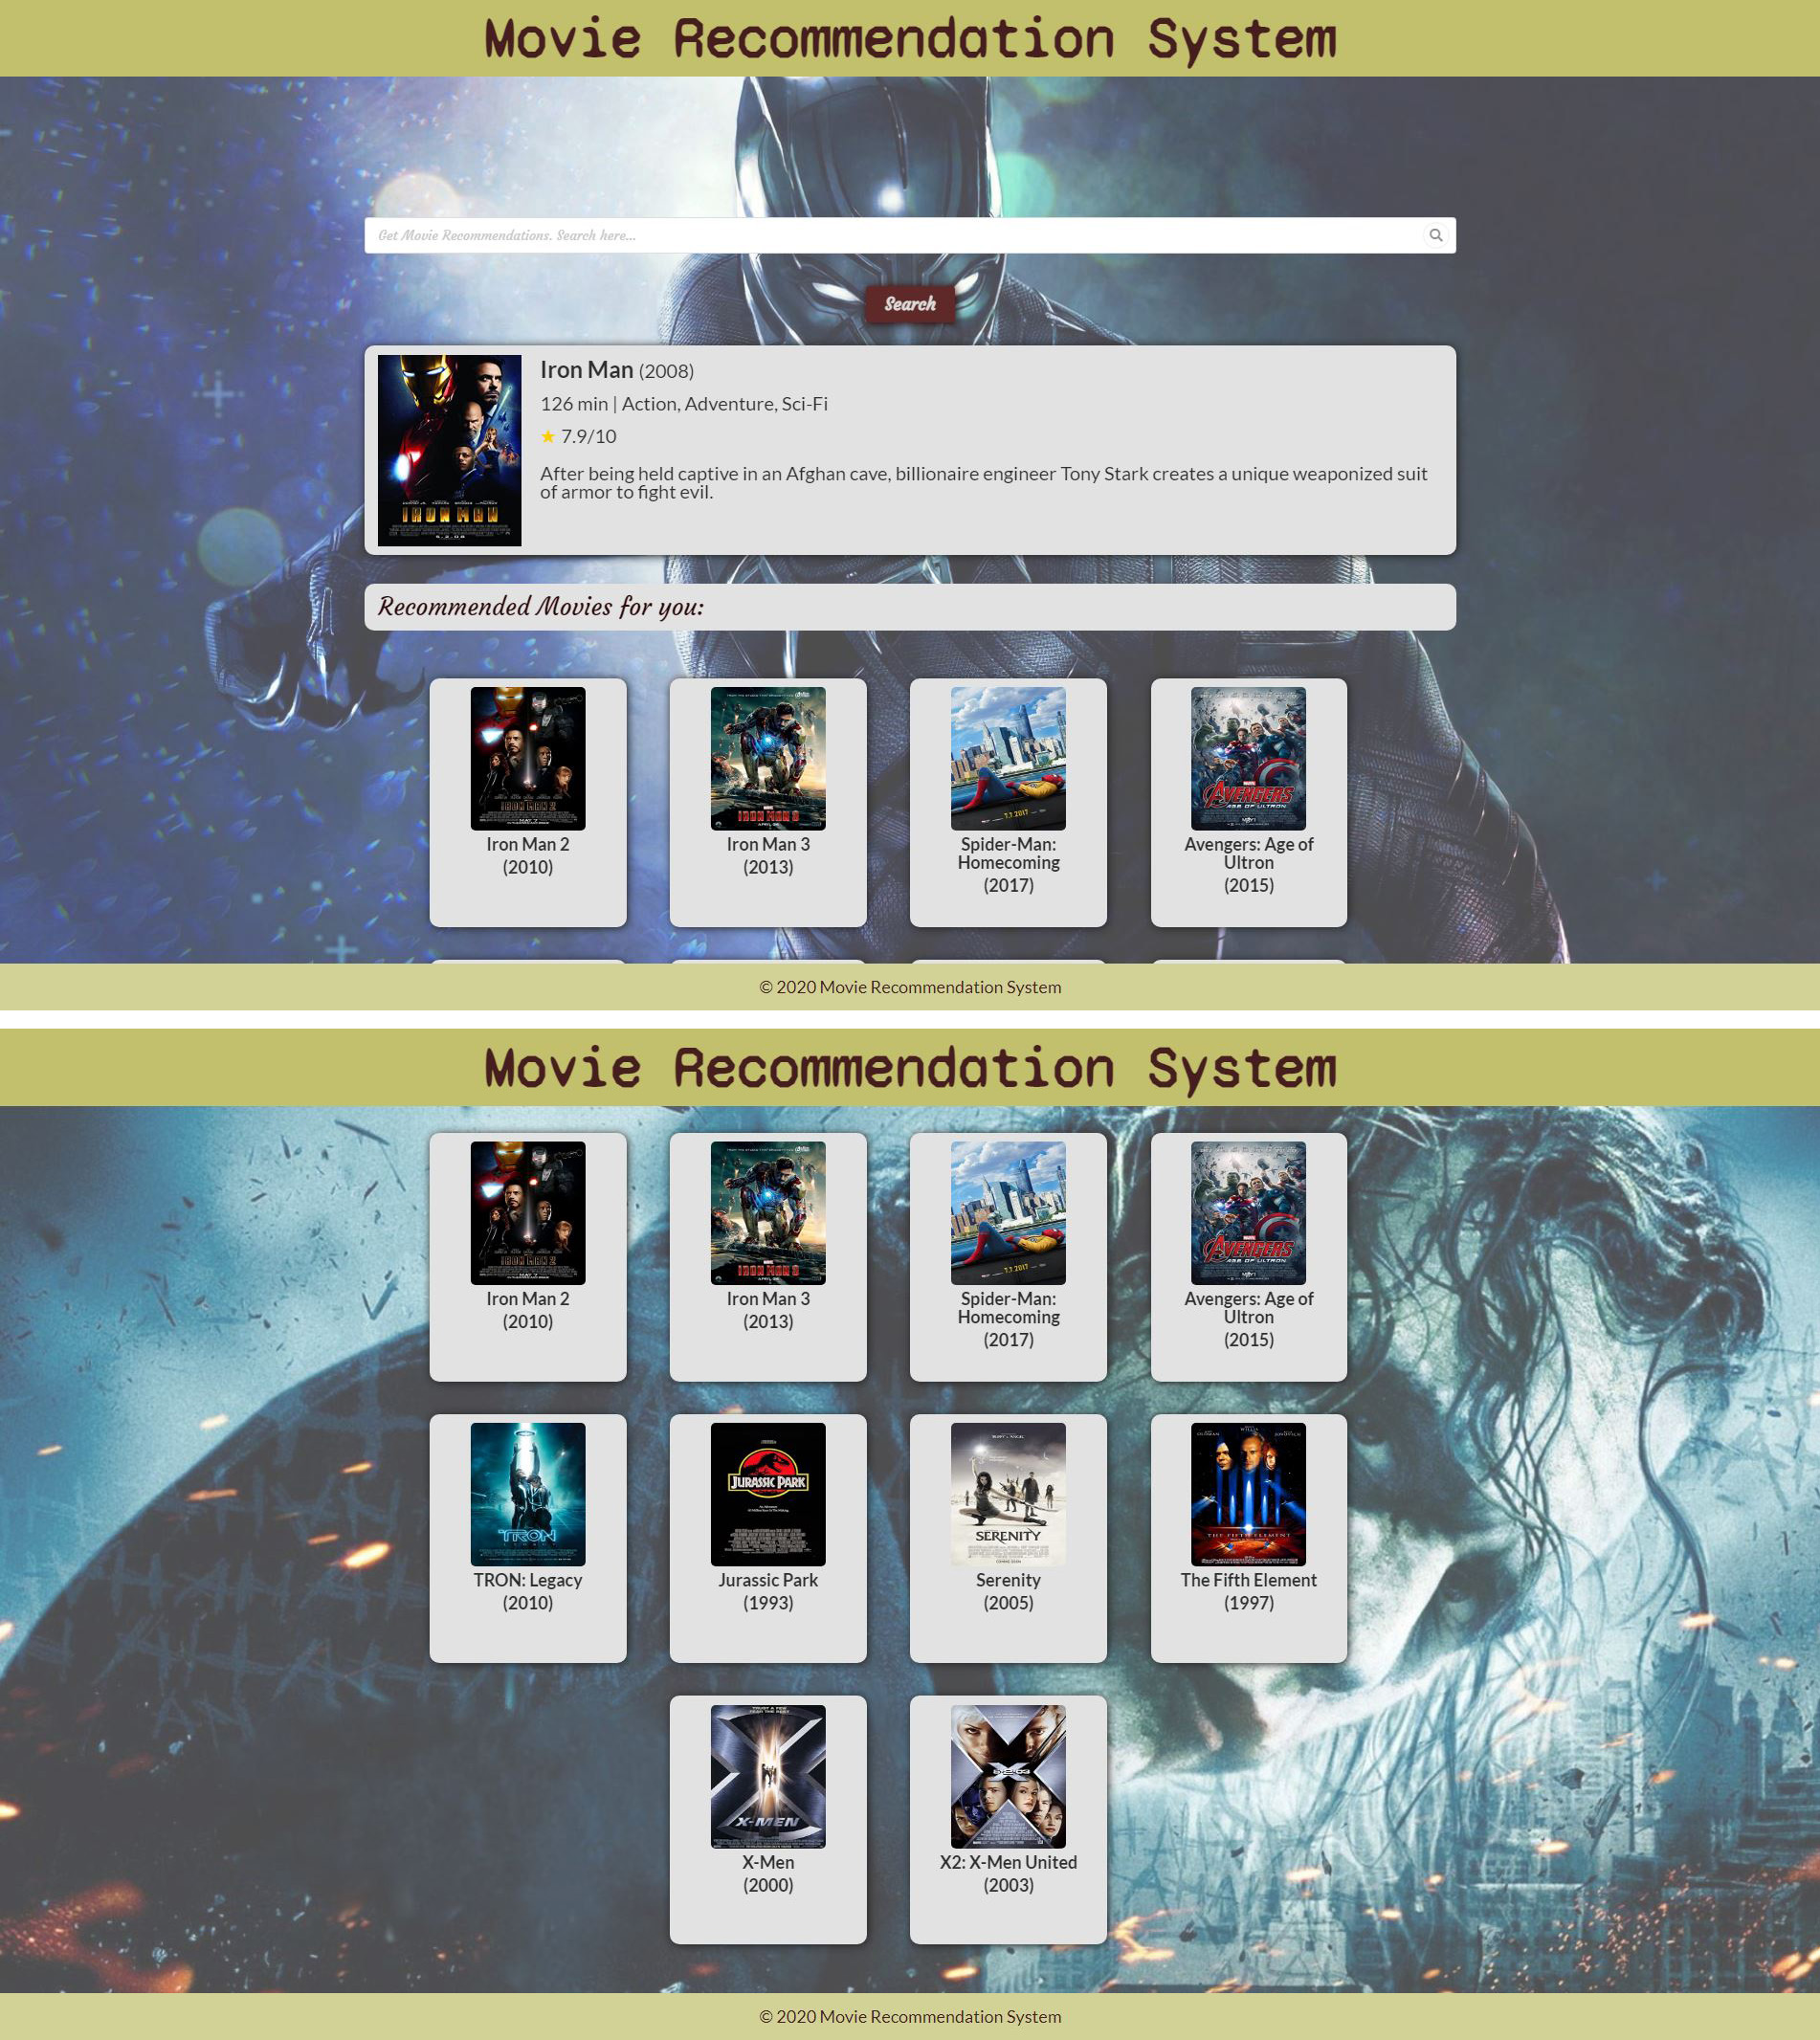
\includegraphics[width=1.0\textwidth]{images/laptop_2.JPG}
	\caption{\textbf{Screenshots of Movie Details and Recommendations on Desktop.} These screenshots show the details of the searched movie i.e "Iron Man" and recommendations for this movie.}
  	\label{fig:laptop-2}
\end{figure}

\begin{figure}[ht]
	\centering
  	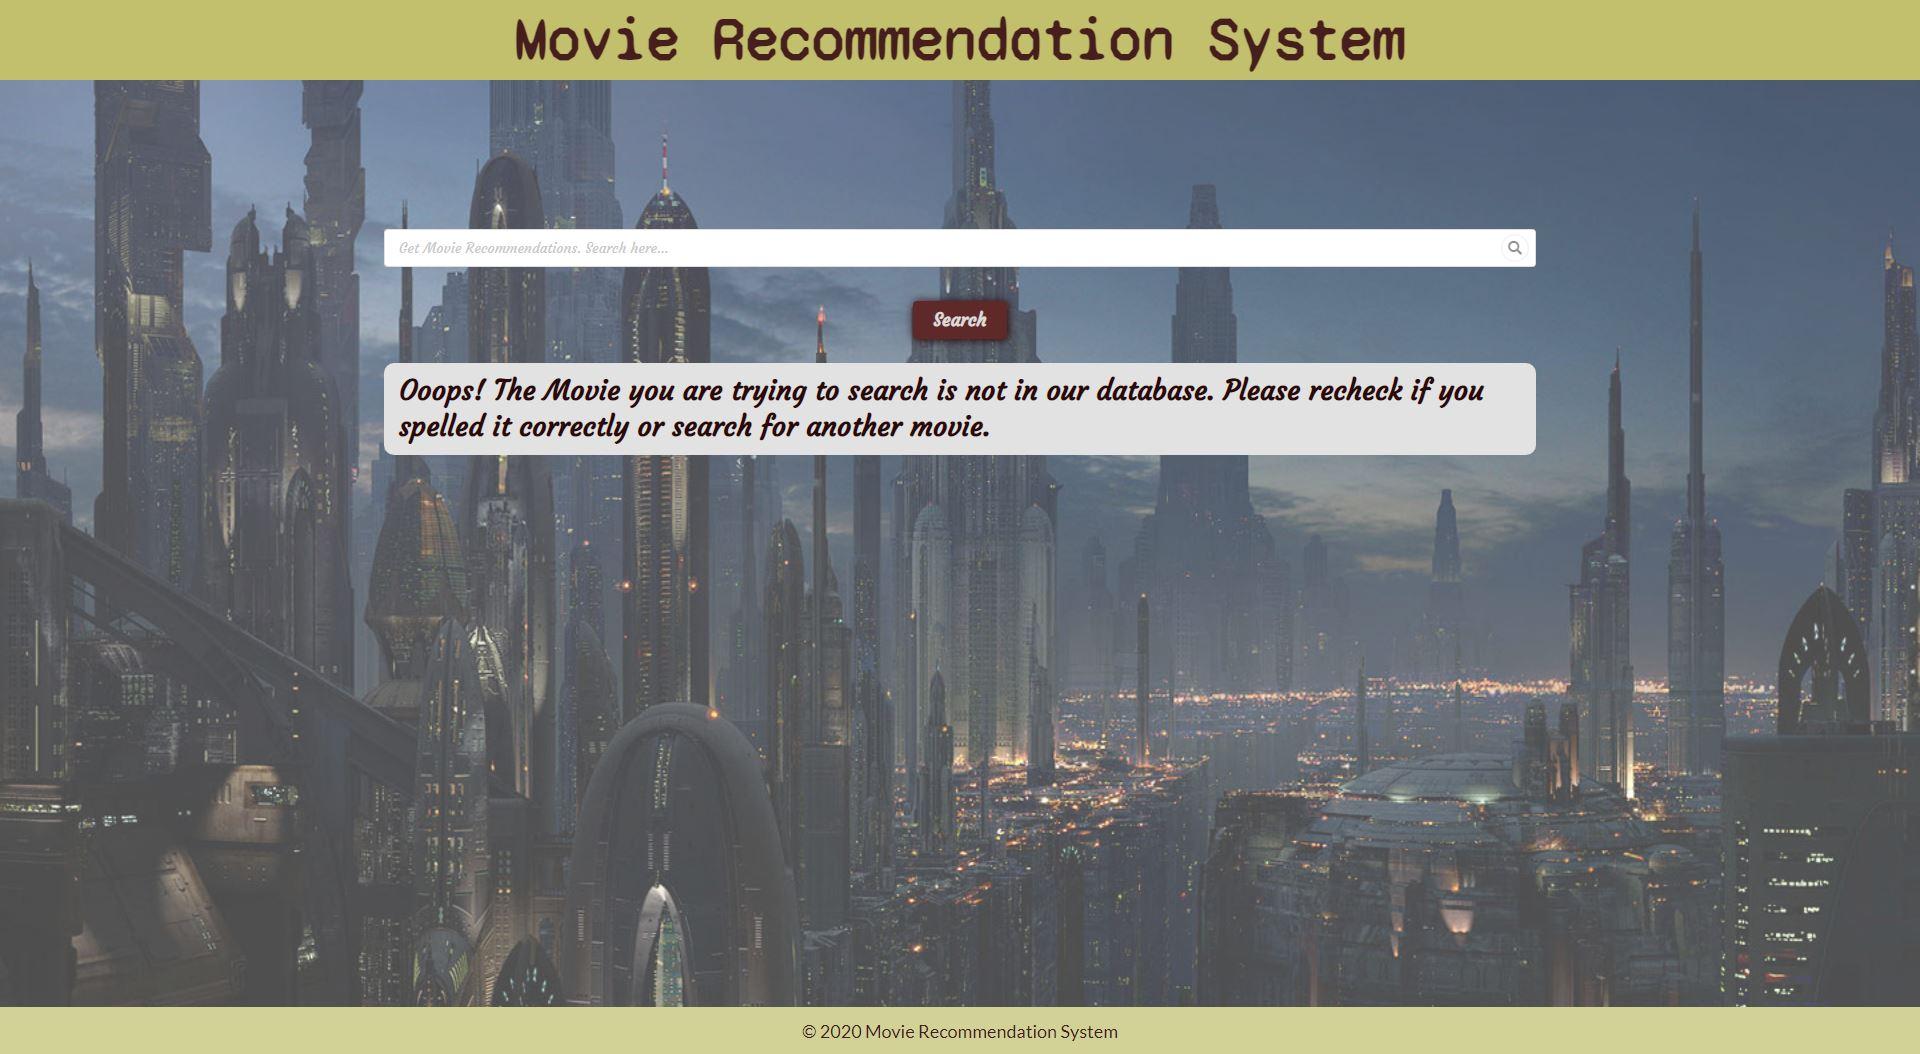
\includegraphics[width=1.0\textwidth]{images/laptop_error.JPG}
	\caption{\textbf{Screenshots of Movie Details and Recommendations on Desktop.} These screenshots show the details of the searched movie i.e "Iron Man" and recommendations for this movie.}
  	\label{fig:laptop-error}
\end{figure}


\subsection{Mobile}

These figures show our project for the Mobile Portrait. Figure \ref{fig:mobile-p-1} shows the first page and movie details after searching a movie. Figure \ref{fig:mobile-p-2} shows some of the recommendations for the searched movie and message for a non-existing movie.

\begin{figure}[ht]
	\centering
  	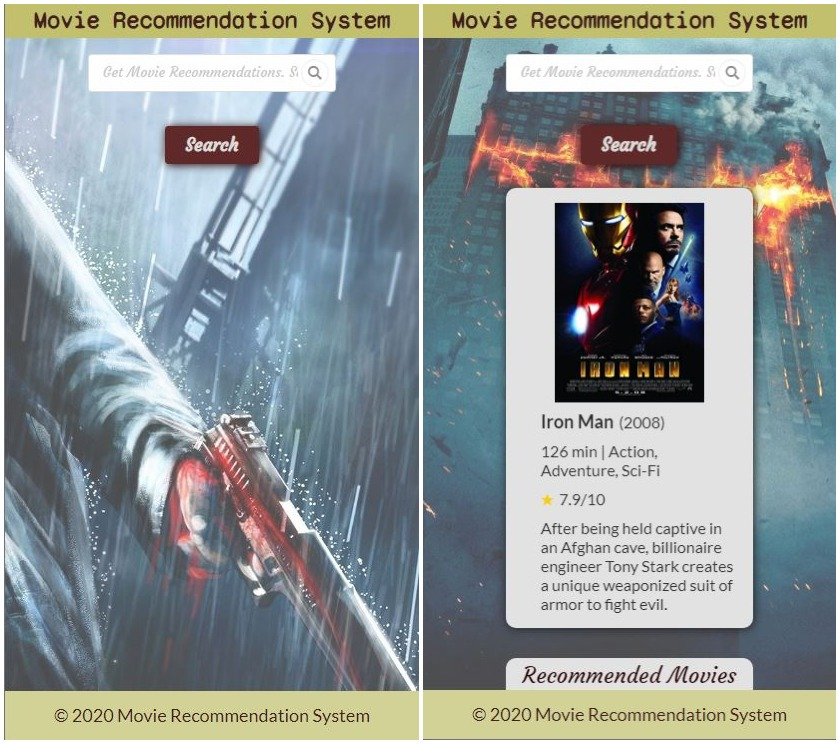
\includegraphics[width=1.0\textwidth]{images/mobile_p_1.JPG}
	\caption{\textbf{Screenshots of First Page and Searched Movie Details for Mobile Portrait.} These screenshots show the first page and user search movie details i.e “Iron Man”.}
  	\label{fig:mobile-p-1}
\end{figure}

\begin{figure}[ht]
	\centering
  	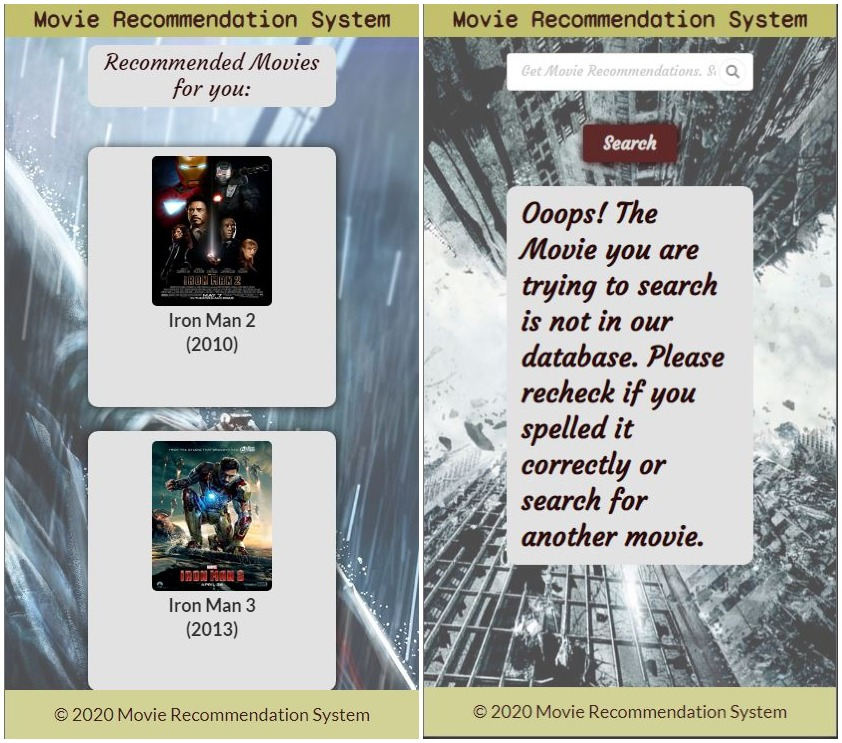
\includegraphics[width=1.0\textwidth]{images/mobile_p_2.JPG}
	\caption{\textbf{Screenshots of the Recommended Movies and Non-Existing Movie Message for Mobile Portrait.} These screenshots show the recommendations for the above searched movie and error message, if the movie does not exist in our database.}
  	\label{fig:mobile-p-2}
\end{figure}

Following figures show our project for the Mobile Landscape. When the user loads the website, it shows the page with search bar and search button as shown in Figure \ref{fig:mobile-l-1}. After the user searches a movie and if that movie exists, the user gets to see the movie details and recommendation as shown in Figure \ref{fig:mobile-l-2} and Figure \ref{fig:mobile-l-3}. Else the user sees the message shown in Figure \ref{fig:mobile-l-error}.

\begin{figure}[ht]
	\centering
  	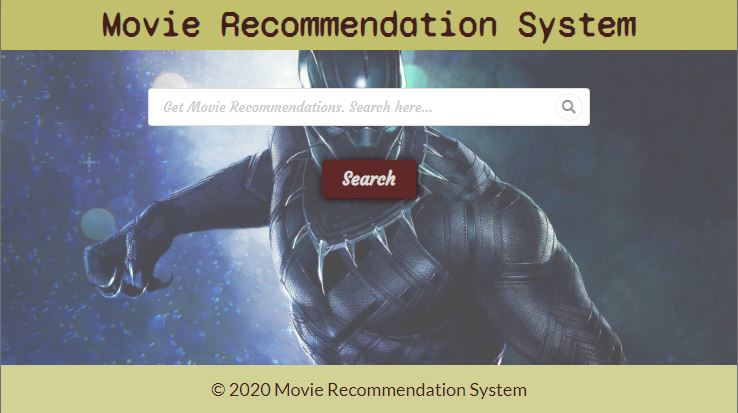
\includegraphics[width=1.0\textwidth]{images/mobile_l_1.JPG}
	\caption{\textbf{Screenshot of First Page for Mobile Landscape.} This figure shows the first page. The user searches the movie name and clicks the search button.}
  	\label{fig:mobile-l-1}
\end{figure}

\begin{figure}[ht]
	\centering
  	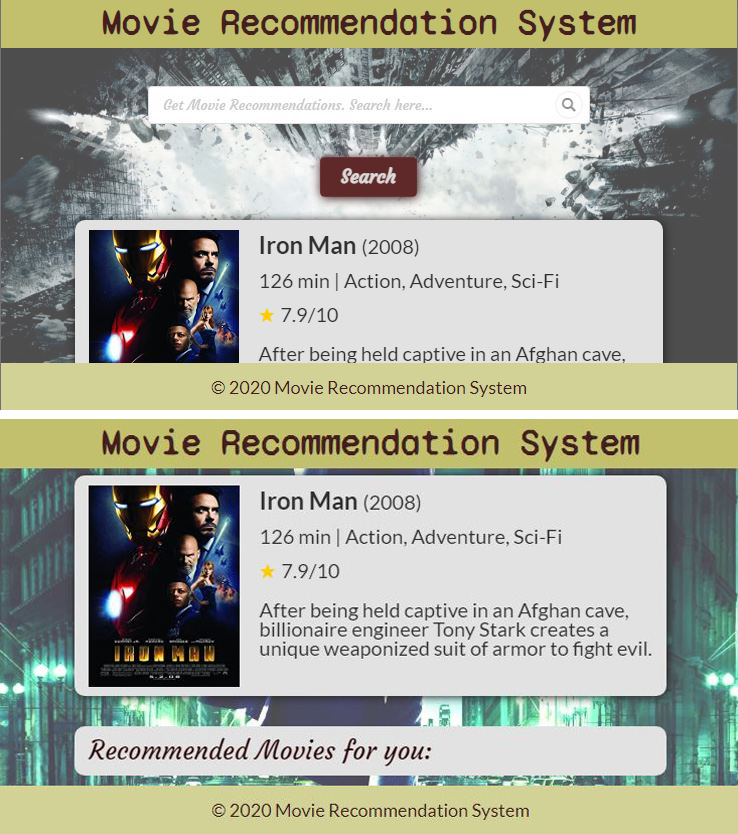
\includegraphics[width=1.0\textwidth]{images/mobile_l_2.JPG}
	\caption{\textbf{Screenshots of Movie Details for Mobile Landscape.} These screenshots show the details of the searched movie.}
  	\label{fig:mobile-l-2}
\end{figure}

\begin{figure}[ht]
	\centering
  	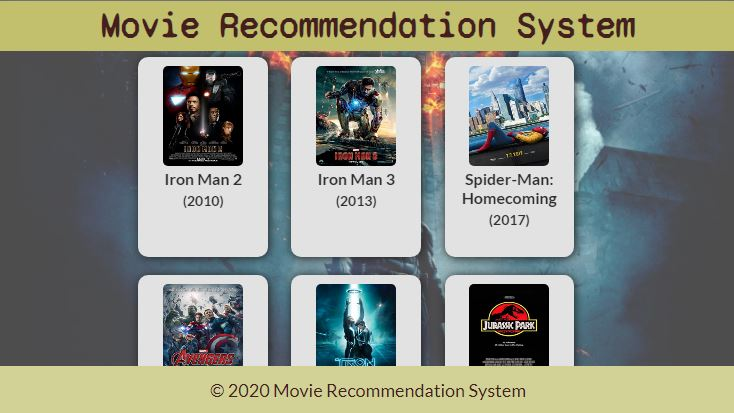
\includegraphics[width=1.0\textwidth]{images/mobile_l_3.JPG}
	\caption{\textbf{Screenshot of Recommended Movies for Mobile Landscape.} This figures shows the recommended movies according to the searched movie "Iron Man".}
  	\label{fig:mobile-l-3}
\end{figure}

\begin{figure}[ht]
	\centering
  	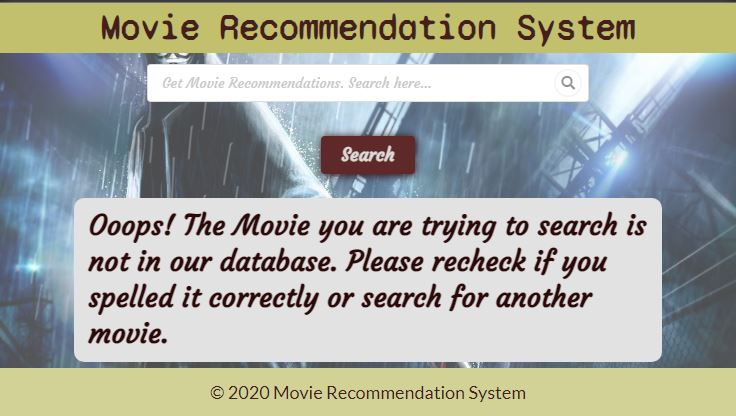
\includegraphics[width=1.0\textwidth]{images/mobile_l_error.JPG}
	\caption{\textbf{Screenshot of Non-existing Movie Message for Mobile Landscape.} This figure shows the error message, if the user searched movie is not in our database.}
  	\label{fig:mobile-l-error}
\end{figure}


\subsection{iPad}

Our project for the iPad is shown in the following figures. Figure \ref{fig:ipad-1} shows the first page and details for the searched movie. Figure \ref{fig:ipad-2} shows the recommendation for the searched movie and message for a non-existing movie.

\begin{figure}[ht]
	\centering
  	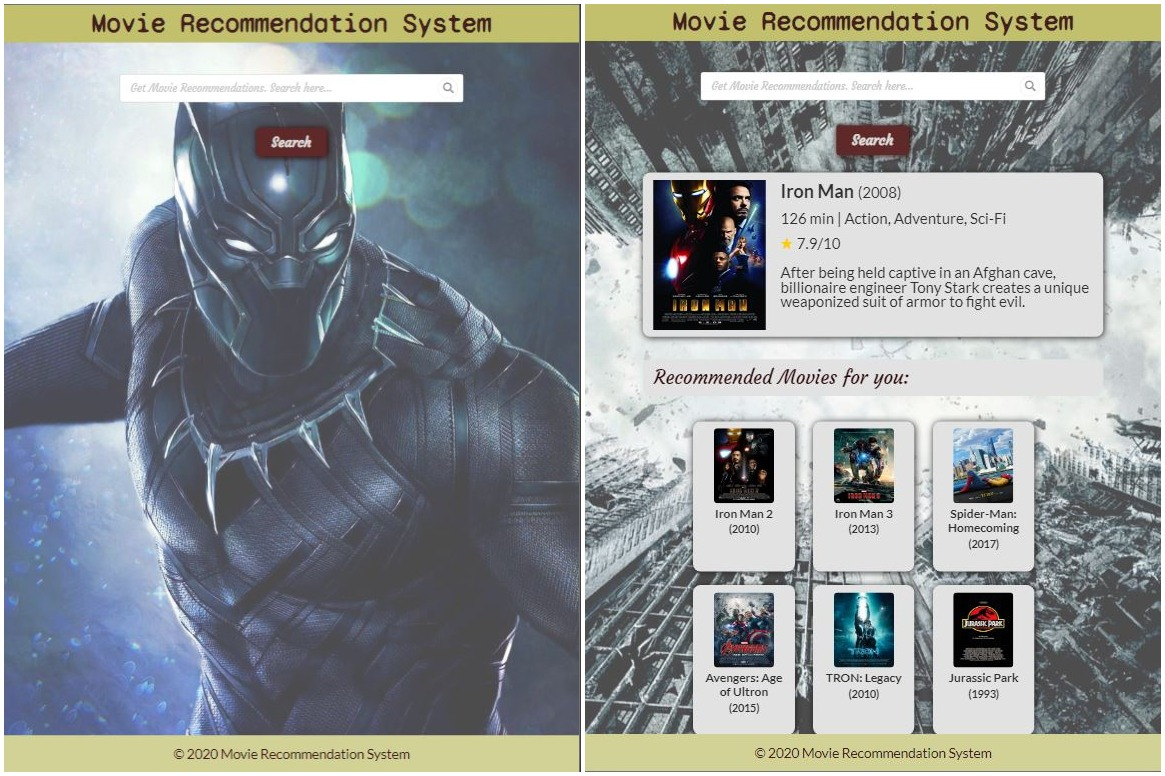
\includegraphics[width=1.0\textwidth]{images/iPad_1.JPG}
	\caption{\textbf{Screenshots of First Page and Movie Details for iPad.} These screenshots show the first page, when the user opens a web page and movie details of the searched movie.}
  	\label{fig:ipad-1}
\end{figure}

\begin{figure}[ht]
	\centering
  	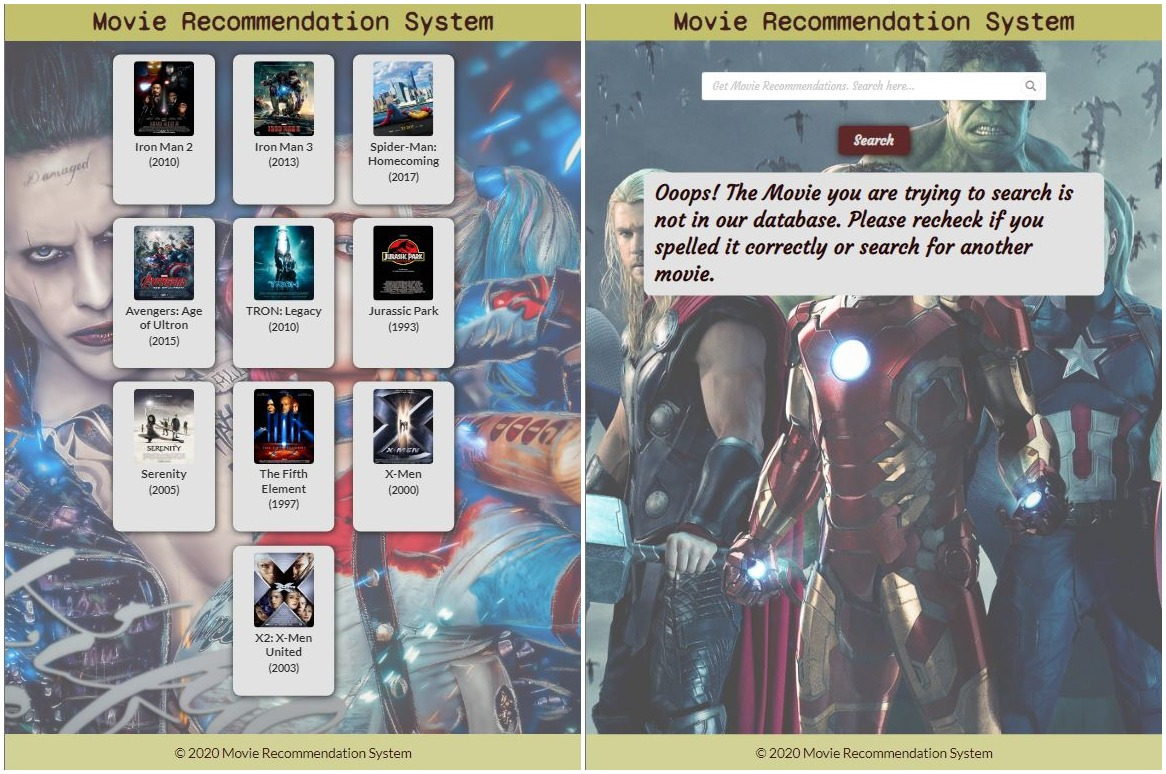
\includegraphics[width=1.0\textwidth]{images/iPad_2.JPG}
	\caption{\textbf{Screenshots of Recommendations and Error Message for iPad.} These screenshots show the recommendations for the searched movie "Iron Man" and error message for the non-existing movie.}
  	\label{fig:ipad-2}
\end{figure}
